% ===== preamble 需要 =====
% \usepackage{graphicx, booktabs, amsmath}

\section{模型的建立与求解}
\subsection{问题一的模型建立与求解}

\subsubsection{建模思路}
将一天按照 $10\,$min 的时间间隔离散为 144 个时段，记时间步长为 $\Delta t=1/6$\,h（10\,min）。
以各时段的外网购电功率、储能充电功率、储能放电功率及弃光功率作为决策变量，
并以各时段末的储电量描述储能设备的状态变化。
首先，根据外网购电、光伏发电、储能充放电与小区负载之间的电能流动关系，建立各时段的功率平衡约束，
以保证微网供电满足小区负载需求；其次，根据储能设备的运行特性，建立储电量状态转移方程，
并设置储电量上下限、最大充放电功率及日循环约束；
最后，以全天外网购电费用最小为目标建立线性规划模型，求解各时段的最优购电及储能充放电策略。

\subsubsection{功率平衡约束}
为保证金微网在各时段的电力供需平衡，外网购电、光伏发电及储能放电共同构成微网的电力供给，
小区负载、储能充电及弃光构成电力消耗。因此，对任一时段 $t$，有
\begin{equation}
p(t)+P_{pv}(t)+u_d(t)=L(t)+u_c(t)+q(t),\qquad t=1,2,\dots,144
\end{equation}
其中，各变量及参数含义见第四章符号说明。该约束保证各时段进入微网的电力与消耗的电力保持平衡。
当光伏发电量超过负载需求及储能可接纳电量时，允许通过 $q(t)$ 表示无法被微网消纳的弃光功率，并满足
\begin{equation}
p(t)\ge 0,\qquad q(t)\ge 0 .
\end{equation}
其中 $p(t)\ge 0$ 表明微网仅从外部电网购电，不考虑向外部电网反向售电。

\subsubsection{储能系统运行约束}
储能设备在相邻时段之间的储电量由上一时段储电量以及当前时段的充、放电行为共同决定。
考虑充放电过程中的能量损耗，建立储能状态转移方程：
\begin{equation}
S(t)=S(t-1)+\eta_c\,u_c(t)\Delta t-\dfrac{u_d(t)\Delta t}{\eta_d},\qquad t=1,2,\dots,144
\end{equation}
其中，$\eta_c=\eta_d=0.9$，$\Delta t=1/6$\,h。充电过程中，实际存入储能设备的电量为 $\eta_c u_c(t)\Delta t$；
放电过程中，为向微网提供 $u_d(t)\Delta t$ 的电量，储能设备实际消耗的电量为 $u_d(t)\Delta t/\eta_d$。

为避免储能设备过度充电或放电，根据题目给出的储电量运行范围，对各时刻储电量设置约束：
\begin{equation}
1200\le S(t)\le 10800,\qquad t=0,1,\dots,144 .
\end{equation}
同时，储能设备最大充放电功率为 5000\,kW，因此有
\begin{equation}
0\le u_c(t)\le 5000,\qquad 0\le u_d(t)\le 5000,\qquad t=1,2,\dots,144 .
\end{equation}
此外，问题一要求储能设备在 0:00 与 24:00 的储电量保持一致，因此设置日循环约束：
\begin{equation}
S(144)=S(0).
\end{equation}
上述约束共同刻画储能设备在一天内的能量状态变化及运行边界，保证所得充放电策略满足储能设备的实际运行要求。

\subsubsection{目标函数}
问题一的优化目标是在满足微网供需平衡及储能运行约束的前提下，使全天从外部电网购电所产生的总费用最小。
设第 $t$ 个时段的外网电价为 $c(t)$，外网购电功率为 $p(t)$，单个时段长度为 $\Delta t=1/6$\,h，
则第 $t$ 个时段的购电量为 $p(t)\Delta t$，相应的购电费用为 $c(t)p(t)\Delta t$。
因此，全天购电总费用的目标函数可表示为
\begin{equation}
\min Z=\sum_{t=1}^{144} c(t)\,p(t)\,\Delta t .
\end{equation}
其中，$Z$ 表示全天购电总费用。通过最小化该目标函数，可在满足各项约束的条件下得到最优日前购电及储能充放电策略。

\subsubsection{模型求解方法}
由上述目标函数及约束条件可知，模型的目标函数与各项约束均为决策变量的线性函数，
因此问题一可归结为线性规划问题。模型共包含 721 个变量，包括 144 个时段的外网购电功率、
储能充电功率、储能放电功率和弃光功率，以及 145 个储能状态变量。
将附件 1 中的分时电价、小区负载及光伏发电预测功率代入模型，
采用 Python 中的 \texttt{scipy.optimize.linprog} 函数并调用 HiGHS 求解器求解，
得到 144 个时段的最优外网购电、储能充放电及储电量变化方案。
由于模型中的外网购电决策变量 $p(t)$ 表示功率，而题目要求输出各 10\,min 时段的购电量，因此按照
\begin{equation}
Q_t=p(t)\Delta t
\end{equation}
将购电功率转换为相应时段的购电量，并据此生成问题一的日前计划购电策略。

\subsubsection{求解结果与分析}
将附件 1 中的电价、小区负载及光伏发电预测数据代入上述模型求解，
得到问题一的最优日前购电及储能调度方案。最优策略下，
全天外网购电量为 59482.70\,kWh，全天购电费用为 35118.60 元，
0:00 与 24:00 储电量均为 8550.00\,kWh，满足日循环约束，且全天弃光量为 0。
题目要求的典型时段购电结果如表~\ref{tab:q1-plan} 所示。

\begin{table}[!htbp]
\caption{微网在指定时间段的购电量及全天的购电量和购电费（情形 A）}\label{tab:q1-plan}
\centering
\begin{tabular}{cccccc}
\toprule
时间段 & 购电量/kWh & 时间段 & 购电量/kWh & 时间段 & 购电量/kWh \\
\midrule
10:00--10:10 & 0.0000 & 12:00--12:10 & 486.4029 & 14:00--14:10 & 0.0000 \\
16:00--16:10 & 394.9315 & 18:00--18:10 & 636.9826 & 20:00--20:10 & 0.0000 \\
\multicolumn{3}{l}{全天购电量/kWh：59482.70} & \multicolumn{3}{l}{全天购电费/元：35118.60} \\
\bottomrule
\end{tabular}
\end{table}

\begin{table}[!htbp]
\caption{储能设备在指定时间段的充放电量及 0:00 和 24:00 的储电量（情形 A）}\label{tab:q1-soc}
\centering
\begin{tabular}{cccccc}
\toprule
时间段 & 充电量/kWh & 放电量/kWh & 时间段 & 充电量/kWh & 放电量/kWh \\
\midrule
0:00--4:00   & 1666.6667 & 0.0000    & 4:00--8:00   & 833.3333  & 5947.4197 \\
8:00--12:00  & 3954.6310 & 2121.4184 & 12:00--16:00 & 6119.3685 & 91.1014 \\
16:00--20:00 & 0.0000    & 5068.6869 & 20:00--24:00 & 8166.6667 & 3571.3131 \\
\multicolumn{3}{l}{0:00 储电量/kWh：8550.0000} & \multicolumn{3}{l}{24:00 储电量/kWh：8550.0000} \\
\bottomrule
\end{tabular}
\end{table}

\begin{figure}[!htbp]
\centering
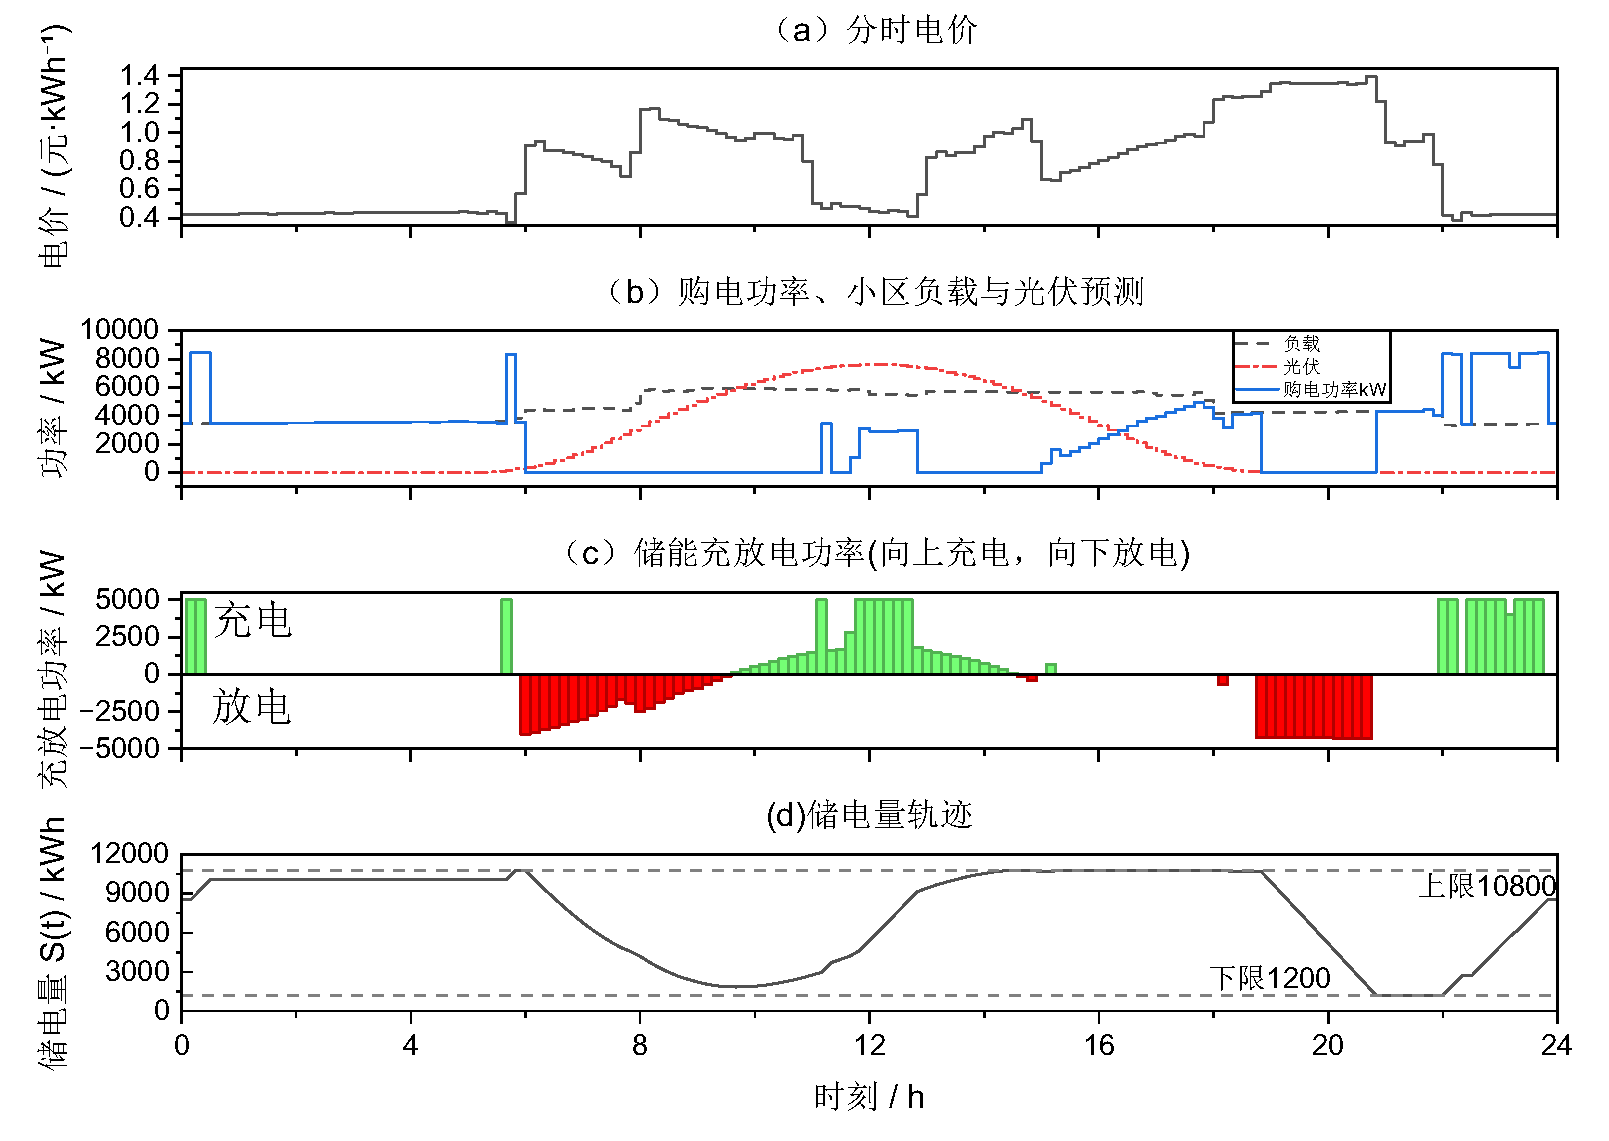
\includegraphics[width=\textwidth]{Q1_CaseA.pdf}
\caption{情形 A（0:00 与 24:00 的储电量由模型自行确定，均为 8550.00\,kWh，全天购电费 35118.60 元）
下微网的最优日前调度结果：(a) 分时电价；(b) 购电功率与小区负载；
(c) 储能充放电功率（向上为充电、向下为放电）；(d) 储电量变化轨迹（虚线为运行上下限 1200 / 10800\,kWh）}
\label{fig:q1-caseA}
\end{figure}

由图~\ref{fig:q1-caseA} 可知，储能设备的充放电行为与分时电价、光伏出力及负荷变化具有明显的协同关系。
在夜间低电价时段，模型通过增加外网购电对储能设备进行充电，为后续高电价时段提供电能；
随着电价上升，储能设备逐步放电，以替代部分高价外网购电；
中午光伏出力较高时，外网购电需求明显降低，同时利用富余光伏及较低价格电能进行储能补充；
在傍晚高电价时段，储能设备再次集中放电，从而降低高价时段的外网购电需求。

从储电量变化曲线可以看出，储能设备全天始终保持在 1200$\sim$10800\,kWh 的允许范围内，
并在日末恢复至与日初相同的 8550\,kWh，说明所得调度方案满足储能容量及日循环约束。
同时，最优方案全天弃光量为 0，表明在当前负荷、光伏出力及储能配置条件下，光伏电能能够得到充分消纳。

需要说明的是，题目要求问题一中储能设备 0:00 与 24:00 的储电量保持一致，
而附录 1 另给出了 2025 年 1 月 1 日 0:00 的储电量为 6000\,kWh。
考虑到问题一描述的是具有固定日内规律的典型日调度，本文以首末储电量相等作为日循环边界条件，
由模型自主确定循环起始储电量，得到 $S(0)=S(24)=8550$\,kWh。
为考察初始储电量取值对结果的影响，进一步设置 $S(0)=S(24)=6000$\,kWh 进行对照求解，
所得全天购电费用由 35118.60 元变为 35126.95 元，仅增加 8.35 元（$+0.024\%$），
全天购电量均为 59482.70\,kWh，表明该边界条件的不同解释对问题一主要结论影响较小，
对照结果如图~\ref{fig:q1-caseB} 所示。

\begin{figure}[!htbp]
\centering
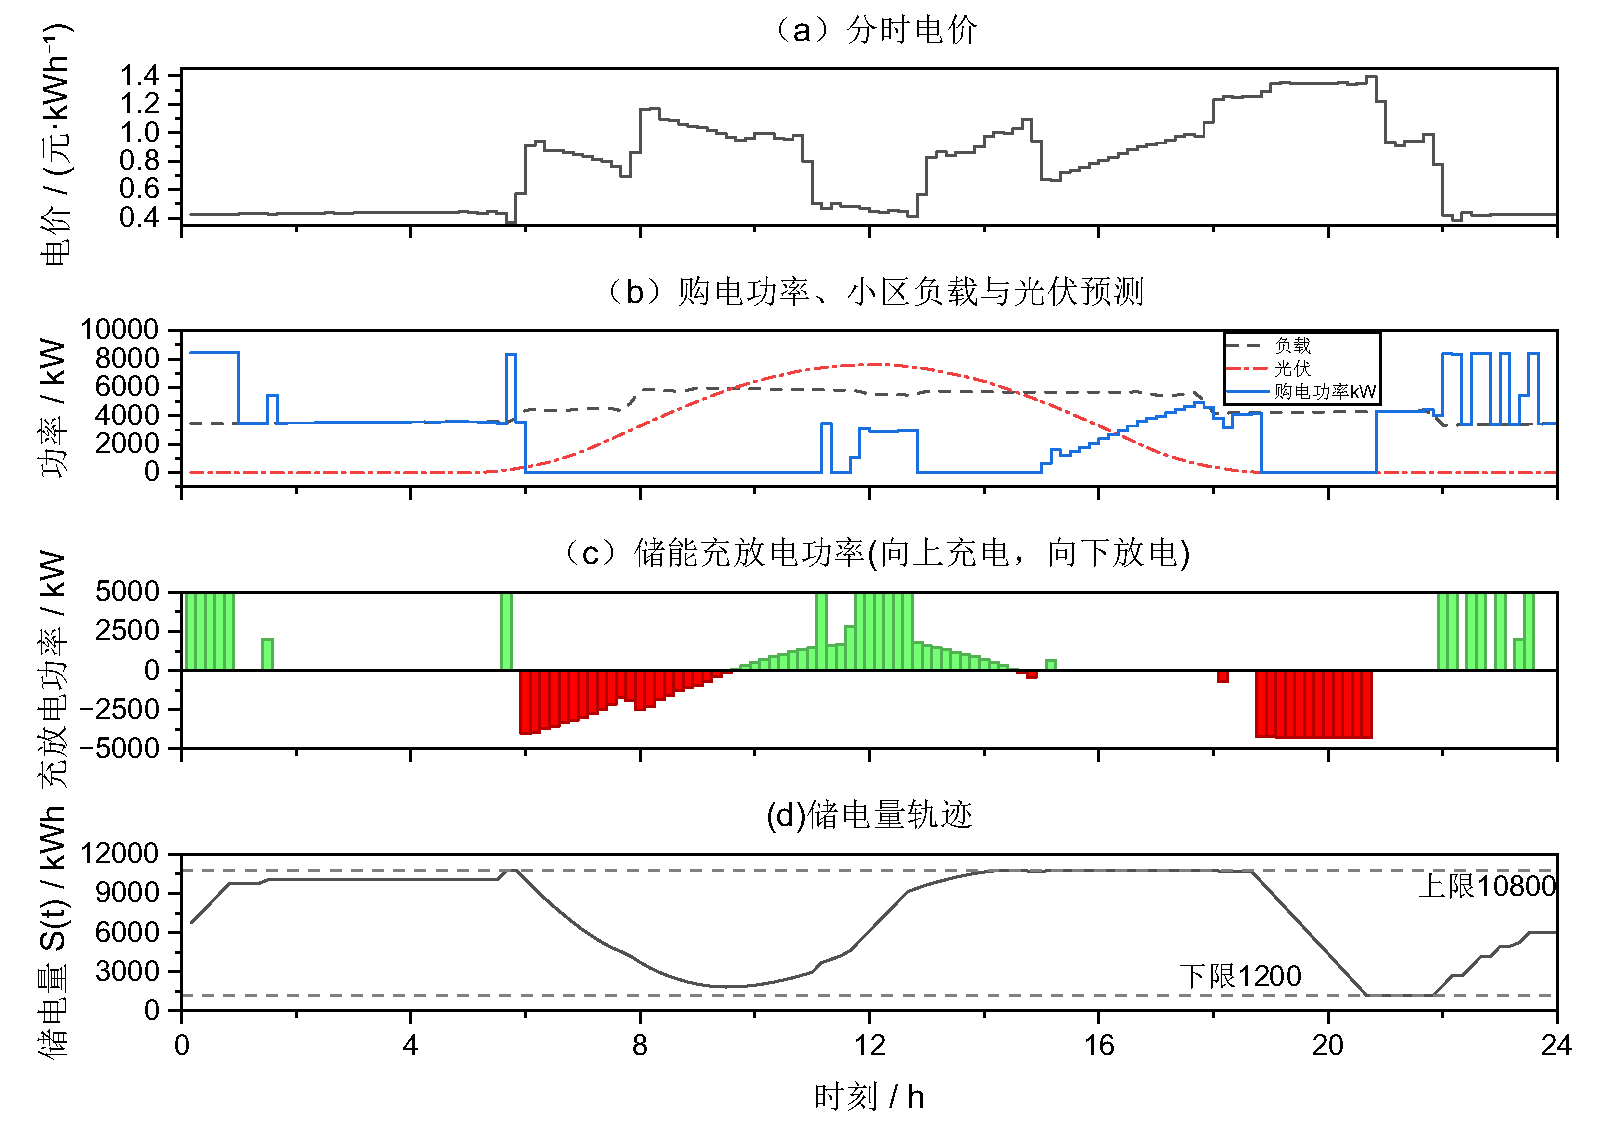
\includegraphics[width=\textwidth]{Q1_CaseB.pdf}
\caption{情形 B（初始储电量固定为 $S(0)=S(24{:}00)=6000.00$\,kWh，全天购电费 35126.95 元，
较情形 A 高 8.35 元）下微网的最优日前调度结果，各子图含义同图~\ref{fig:q1-caseA}}
\label{fig:q1-caseB}
\end{figure}
